% !TEX TS-program = XeLaTeX
% use the following command: 
% all document files must be coded in UTF-8
\documentclass{textolivre}
% for anonymous submission
%\documentclass[anonymous]{textolivre}
% to create HTML use 
%\documentclass{textolivre-html}
% See more information on the repository: https://github.com/leolca/textolivre

% Metadata
\begin{filecontents*}[overwrite]{article.xmpdata}
    \Title{Uso de las TIC y atención a la diversidad en los tiempos de  la COVID}
    \Author{Blas González Alba}
    \Language{es}
    \Keywords{palavra1 \sep palavra dois \sep palavra-três \sep palavra4}
    \Journaltitle{Texto Livre}
    \Journalnumber{1983-3652}
    \Volume{14}
    \Issue{2}
    \Firstpage{1}
    \Lastpage{12}
    \Doi{10.35699/1983-3652.2021.33578}

    \setRGBcolorprofile{sRGB_IEC61966-2-1_black_scaled.icc}
            {sRGB_IEC61966-2-1_black_scaled}
            {sRGB IEC61966 v2.1 with black scaling}
            {http://www.color.org}
\end{filecontents*}

% used to create dummy text for the template file
\definecolor{dark-gray}{gray}{0.35} % color used to display dummy texts
\usepackage{lipsum}
\SetLipsumParListSurrounders{\colorlet{oldcolor}{.}\color{dark-gray}}{\color{oldcolor}}

% used here only to provide the XeLaTeX and BibTeX logos
\usepackage{hologo}

% used in this example to provide source code environment
%\crefname{lstlisting}{lista}{listas}
%\Crefname{lstlisting}{Lista}{Listas}
%\usepackage{listings}
%\renewcommand\lstlistingname{Lista}
%\lstset{language=bash,
        breaklines=true,
        basicstyle=\linespread{1}\small\ttfamily,
        numbers=none,xleftmargin=0.5cm,
        frame=none,
        framexleftmargin=0.5em,
        framexrightmargin=0.5em,
        showstringspaces=false,
        upquote=true,
        commentstyle=\color{gray},
        literate=%
           {á}{{\'a}}1 {é}{{\'e}}1 {í}{{\'i}}1 {ó}{{\'o}}1 {ú}{{\'u}}1 
           {à}{{\`a}}1 {è}{{\`e}}1 {ì}{{\`i}}1 {ò}{{\`o}}1 {ù}{{\`u}}1
           {ã}{{\~a}}1 {ẽ}{{\~e}}1 {ĩ}{{\~i}}1 {õ}{{\~o}}1 {ũ}{{\~u}}1
           {â}{{\^a}}1 {ê}{{\^e}}1 {î}{{\^i}}1 {ô}{{\^o}}1 {û}{{\^u}}1
           {ä}{{\"a}}1 {ë}{{\"e}}1 {ï}{{\"i}}1 {ö}{{\"o}}1 {ü}{{\"u}}1
           {Á}{{\'A}}1 {É}{{\'E}}1 {Í}{{\'I}}1 {Ó}{{\'O}}1 {Ú}{{\'U}}1
           {À}{{\`A}}1 {È}{{\`E}}1 {Ì}{{\`I}}1 {Ò}{{\`O}}1 {Ù}{{\`U}}1
           {Ã}{{\~A}}1 {Ẽ}{{\~E}}1 {Ũ}{{\~u}}1 {Õ}{{\~O}}1 {Ũ}{{\~U}}1
           {Â}{{\^A}}1 {Ê}{{\^E}}1 {Î}{{\^I}}1 {Ô}{{\^O}}1 {Û}{{\^U}}1
           {Ä}{{\"A}}1 {Ë}{{\"E}}1 {Ï}{{\"I}}1 {Ö}{{\"O}}1 {Ü}{{\"U}}1
           {ç}{{\c{c}}}1 {Ç}{{\c{C}}}1
}


\journalname{Texto Livre}
\thevolume{14}
\thenumber{2}
\theyear{2021}
\receiveddate{\DTMdisplaydate{2020}{12}{11}{-1}} % YYYY MM DD
\accepteddate{\DTMdisplaydate{2021}{02}{28}{-1}}
\publisheddate{\DTMdisplaydate{2021}{6}{15}{-1}}
% Corresponding author
\corrauthor{Blas González Alba}
% DOI
\articledoi{10.35699/1983-3652.2021.33578}
% list of available sesscions in the journal: articles, dossier, reports, essays, reviews, interviews, editorial
\articlesessionname{dossier}
% Abbreviated author list for the running footer
\runningauthor{González Alba}
\editorname{Anna Izabella Miranda Pereira}

\title{Uso de las TIC y atención a la diversidad en los tiempos de  la COVID}
\othertitle{Uso das TIC e atenção à diversidade em tempos de  COVID}
\othertitle{Use of ICT and attention to diversity in times of COVID}
% if there is a third language title, add here:
%\othertitle{Artikelvorlage zur Einreichung beim Texto Livre Journal}

\author[1]{Blas González Alba \orcid{0000-0002-4769-6522} \thanks{Email: \url{blas@uma.es}}}

\affil[1]{Universidad de Málaga, Facultad de
Ciencias de la Educación, Departamento de didáctica y organización
escolar. Málaga, Andalucía y España.}

\addbibresource{article.bib}
% use biber instead of bibtex
% $ biber tl-article-template

% set language of the article
\setdefaultlanguage{spanish}
\setotherlanguage{portuguese}
\setotherlanguage{english}

% for spanish, use:
%\setdefaultlanguage{spanish}
%\gappto\captionsspanish{\renewcommand{\tablename}{Tabla}} % use 'Tabla' instead of 'Cuadro'
%\AfterEndPreamble{\crefname{table}{tabla}{tablas}}

% for languages that use special fonts, you must provide the typeface that will be used
% \setotherlanguage{arabic}
% \newfontfamily\arabicfont[Script=Arabic]{Amiri}
% \newfontfamily\arabicfontsf[Script=Arabic]{Amiri}
% \newfontfamily\arabicfonttt[Script=Arabic]{Amiri}
%
% in the article, to add arabic text use: \textlang{arabic}{ ... }

% to use emoticons in your manuscript
% https://stackoverflow.com/questions/190145/how-to-insert-emoticons-in-latex/57076064
% using font Symbola, which has full support
% the font may be downloaded at:
% https://dn-works.com/ufas/
% add to preamble:
% \newfontfamily\Symbola{Symbola}
% in the text use:
% {\Symbola }

% reference itens in a descriptive list using their labels instead of numbers
% insert the code below in the preambule:
\makeatletter
\let\orgdescriptionlabel\descriptionlabel
\renewcommand*{\descriptionlabel}[1]{%
  \let\orglabel\label
  \let\label\@gobble
  \phantomsection
  \edef\@currentlabel{#1\unskip}%
  \let\label\orglabel
  \orgdescriptionlabel{#1}%
}
\makeatother
%
% in your document, use as illustraded here:
%\begin{description}
%  \item[first\label{itm1}] this is only an example;
%  % ...  add more items
%\end{description}
 

% custom epigraph - BEGIN 
%%% https://tex.stackexchange.com/questions/193178/specific-epigraph-style
\usepackage{epigraph}
\renewcommand\textflush{flushright}
\makeatletter
\newlength\epitextskip
\pretocmd{\@epitext}{\em}{}{}
\apptocmd{\@epitext}{\em}{}{}
\patchcmd{\epigraph}{\@epitext{#1}\\}{\@epitext{#1}\\[\epitextskip]}{}{}
\makeatother
\setlength\epigraphrule{0pt}
\setlength\epitextskip{0.5ex}
\setlength\epigraphwidth{.7\textwidth}
% custom epigraph - END


% if you use multirows in a table, include the multirow package
\usepackage{multirow}

% add line numbers for submission
%\usepackage{lineno}
%\linenumbers

\begin{document}
\maketitle

\begin{polyabstract}
\begin{abstract}
La pandemia provocada por la COVID-19 ha configurado un escenario escolar caracterizado por procesos de enseñanza-aprendizaje vinculados exclusivamente con el uso de dispositivos tecnológicos y aplicaciones virtuales. Con el propósito de conocer la experiencia del profesorado andaluz de Pedagogía Terapéutica durante el periodo de confinamiento con el alumnado con necesidades educativas y el uso de las nuevas tecnologías, hemos planteado una investigación cualitativa. A partir de entrevistas individuales y grupos focales, 37 maestros y maestras de Pedagogía Terapéutica de la comunidad autónoma de Andalucía han expresado las limitaciones personales, de recursos tecnológicos y formativas y las dificultades encontradas para atender a su alumnado con necesidades del mismo modo en el que lo venían haciendo antes del confinamiento. Esta investigación pone de relieve que desde los centros educativos se ha de mejorar y ampliar la formación del alumnado en el uso de dispositivos y herramientas TIC, especialmente la del alumnado con necesidades educativas, y que necesitamos mejorar la accesibilidad de las aplicaciones y dispositivos tecnológicos con el propósito de que se adapten a las características del alumnado con necesidades educativas. 

\keywords{COVID-19 \sep alumnado con necesidades educativas \sep tecnologías de la información y la comunicación}
\end{abstract}

\begin{portuguese}
\begin{abstract}
A pandemia provocada pelo COVID-19 configurou um ambiente escolar caracterizado por processos de ensino-aprendizagem vinculados exclusivamente ao uso de dispositivos tecnológicos e aplicativos virtuais. Com o objetivo de conhecer a experiência do professor de educação especial durante o período de confinamento com alunos com necessidades educacionais e uso de novas tecnologias, propomos uma investigação qualitativa. A partir de entrevistas individuais e grupos focais, 37 professores de educação especial da comunidade autônoma de Andaluzia expressaram as limitações pessoais, recursos tecnológicos e formativos e as dificuldades encontradas para atender às necessidades de seus alunos da mesma forma como faziam antes do confinamento. Esta pesquisa destaca que os centros educacionais devem melhorar e ampliar a formação dos alunos no uso de dispositivos e ferramentas TIC, especialmente de alunos com necessidades educacionais, e que precisamos melhorar a acessibilidade de aplicativos e dispositivos tecnológicos para que eles possam se adaptar às características dos alunos com necessidades educacionais.

\keywords{COVID-19 \sep alunos com necessidades educacionais \sep Tecnologia da informação e comunicação}

\end{abstract}
\end{portuguese}

\begin{english}
\begin{abstract}
The pandemic caused by COVID-19 has configured a school characterized by teaching-learning processes exclusively linked to the use of technological devices and virtual applications. The aim of this study was to investigate the experience of the Andalusian special education teachers during the period of confinement with students who have educational needs and the use of new technologies. For doing so, we have developed a qualitative investigation. Through individual interviews and focus groups, 37 special education teachers of the autonomous community of Andalusia have expressed the personal limitations, technological and training resources and the difficulties found to attend their students with special needs in the same way in which they had been doing it before confinement. This research highlights that educational centers have to improve and expand the training of students in the use of ICT devices and tools, especially in students with educational needs, and that we need to improve the accessibility of applications and technological devices so they can adapt to the characteristics of students with special educational needs.

\keywords{COVID-19 \sep students with educational needs \sep Technology of the information and communication}

\end{abstract}
\end{english}

% if there is another abstract, insert it here using the same scheme
\end{polyabstract}


\section{Introducción}\label{intro}
El cierre de los centros educativos, y, por tanto, la cancelación de las actividades educativas presenciales como consecuencia del coronavirus SARS-CoV-2 o COVID-19, ha configurado un escenario educativo caracterizado por prácticas de enseñanza-aprendizaje telemáticas \cite{menendez2020}. %(MENÉNDEZ; FIGARES, 2020)
Según datos de \textcite{unicef2020}, %UNICEF (2020)
esta situación ha afectado en España a más de 10.3 millones de estudiantes y a 900.000 profesores y profesoras aproximadamente.

Este nuevo escenario, que ha requerido de un esfuerzo por parte del profesorado — adaptar los contenidos, la organización y las metodologías —, de las familias — responder a las demandas escolares — \cite{rogero2020} %(ROGERO, 2020) 
y del alumnado — desarrollar habilidades y competencias de autogestión y la autorregulación — \cite{munoz2020}, %(MUÑOZ; LLUCH, 2020)
ha sido más complejo para el entramado educativo que ha rodeado al alumnado con necesidades específicas de apoyo educativo (NEAE) \cite{murillo2020}. %(MURILLO; DUCK, 2020). 
En el caso de España, esta situación ha dibujado un escenario acotado temporalmente que podemos denominar situación de confinamiento. 
	
Este periodo abarca desde el día 16 de marzo de 2020, fecha en la que se decretó el estado de alarma \cite{realdecreto}, %(REAL DECRETO 463/2020 de 14 de marzo)
hasta el 22 de junio de 2020 con la finalización del “estado de alarma”. Este nuevo escenario ha desencadenado un proceso de transición en el ámbito educativo en el que las tecnologías de la información y la comunicación han sido imprescindibles para la docencia virtual, el envío y recepción de material didáctico, la comunicación entre el profesorado, con el alumnado y familias, la evaluación, las reuniones del profesorado, entre otras. 

\section{Periodo de confinamiento y atención educativa}
La situación de confinamiento ha configurado un nuevo panorama educativo en el que la utilización de las tecnologías aplicadas a la educación ha tenido una importancia capital \cite{ruiz2020}. %(RUIZ; TAMAYO; MONTIEL, 2020)
Como apuntan \textcite{menendez2020}, %Menéndez y Figares (2020)
durante el confinamiento las nuevas tecnologías han permitido a docentes y discentes intercambiar material didáctico e interactuar en aulas virtuales, posibilitando, por parte del profesorado, el envío, seguimiento y evaluación de las actividades propuestas. 

No obstante, la irrupción de la educación a distancia producto de la emergencia, ha dejado al descubierto la brecha digital existente entre las escuelas y sus docentes \cite[p. 12]{murillo2020}, %(MURILLO; DUK, 2020, p.12)
revelando que, a pesar de los esfuerzos realizados por docentes, familias y alumnado \cite{rogero2020}, %(ROGERO, 2020)
la educación no universitaria está diseñada para la presencialidad \cite{cabreraperez2020} %(CABRERA; PÉREZ; SANTANA, 2020)
y que la comunidad educativa no estaba preparada para asumir procesos de enseñanza y aprendizaje virtuales \cite{penate2020}. %(PEÑATE, 2020)
Es decir, la situación de confinamiento ha descubierto (1) una brecha de acceso — profesorado y familias que no tienen acceso a internet —, (2) una brecha de uso — relacionada con el conocimiento en el uso de tecnologías para la educación virtual — y, (3) una brecha escolar — desconexión entre los centros educativos y la sociedad — \cite{cotec2020}. %(COTEC, 2020) 

Durante el periodo de confinamiento obligatorio han sido muchos los estudiantes que no han dispuesto de recursos y condiciones materiales — conexión a internet y dispositivos informáticos — \cite{menendez2020, rogero2020}, %(MENÉNDEZ; FIGARES, 2020; ROGERO, 2020)
ambientales y espaciales para afrontar procesos de aprendizaje virtuales \cite{fernandez2020, murillo2020}, %(FERNÁNDEZ, 2020; MURILLO; DUK, 2020)
situación que ha contribuido a incrementar la brecha digital entre las familias más desfavorecidas \cite{albala2020, sadio2020}, %(ALBALÁ; GUIDO, 2020; SADIO; ORTIZ; MORENO; BERNABÉ; LÓPEZ, 2020) 
y/o con hijos con discapacidad \cite{berastegui2020}. %(BERASTEGUI, 2020)
En este sentido, y como muestra el estudio desarrollado por \textcite{cabreraperez2020}, %Cabrera, Pérez y Santana (2020)
al menos un 10\% del alumnado, y hasta el 20\%, en algunas comunidades autónomas, no han tenido dispositivos electrónicos y acceso a una conexión de red durante este periodo. 

Esta situación ha obligado a muchas familias a tener que compartir dispositivos o dotarse de recursos informáticos para proseguir el curso escolar \cite{munoz2020}. %(MUÑOZ; LLUCH, 2020)
Así mismo, y como señalan algunos organismos internacionales como la 
%\cite{unesco2016}, %UNESCO (2020)
%\cite{unicef2020} %UNICEF (2020) 
%o la \cite{ocde2020}, %OCDE (2020)
\textcite{unesco2016,unicef2020,ocde2020}
la brecha digital ha venido acompañada de una “brecha familiar” que ha visibilizado que las familias con menos formación han presentado mayores dificultades para ayudar a sus hijos e hijas en las tareas escolares \cite{cabrera2020}. %(CABRERA, 2020).

Sin lugar a duda, el confinamiento ha transformado la realidad educativa y ha construido un escenario en el que las plataformas digitales de aprendizaje y multiconferencia, los correos electrónicos, los recursos online, entre otros, se han convertido en las nuevas herramientas de enseñanza-aprendizaje \cite{menendez2020}, %(MENÉNDEZ; FIGARES, 2020)
obligando al profesorado a adaptar los contenidos y las metodologías y al alumnado a responder a las demandas escolares a través de estas tecnologías \cite{rogero2020}. %(ROGERO, 2020)
Esta situación ha revelado que (1) un buen docente no tiene por qué serlo también utilizando medios telemáticos \cite{fernandezdomingues2020}; %(FERNÁNDEZ; DOMÍNGUEZ; MARTÍNEZ, 2020)
(2) existe poco conocimiento por parte del profesorado en el uso de medios de enseñanza-aprendizaje virtual \cite{rogero2020}; %(ROGERO, 2020)
y, (3) que el empleo de herramientas tecnológicas se relaciona con las visiones, experiencias, creencias y perspectivas del profesorado \cite{marin2020}. %(MARÍN; VAGENA; RUBIO, 2020).

\section{La atención a la diversidad durante el periodo de confinamiento}
La atención escolar y educativa del alumnado diagnosticado con Necesidades Específicas de Apoyo Educativo (NEAE) a lo largo del periodo anterior a la COVID-19 se ha caracterizado generalmente por promover actuaciones de exclusión escolar en un marco normativo inclusivo, esto es, por desarrollar acciones educativas fuera del aula ordinaria \cite{gonzalescortesmanas2020, manasgonzalescortes2020, morina2010} %(GONZÁLEZ; CORTÉS; MAÑAS, 2020; MAÑAS; GONZÁLEZ; CORTÉS, 2020; MORIÑA, 2010) 
o dentro del aula ordinaria pero con un currículum diferente al de sus compañeros \cite{arnaiz2011}. %(ARNAIZ, 2011). 

Si esta situación ya era preocupante, el confinamiento la ha agravado, pues ha supuesto una experiencia limitante en las opciones de inclusión y en el desarrollo y aprendizaje del alumnado con NEAE. Esto se ha debido a que no todo el alumnado se ha adaptado del mismo modo a este nuevo escenario de aprendizaje virtual, lo que ha supuesto un nuevo riesgo de exclusión y desigualdad social para algunos estudiantes \cite{cabrera2020, echeita2020}, %(CABRERA, 2020; ECHEITA, 2020)
principalmente para el alumnado cuyas características personales, físicas, comunicativas…, o dificultades de aprendizaje han requerido de una atención educativa diferente a la ordinaria \cite{menendez2020}, %(MENÉNDEZ; FIGARES, 2020)
es decir, para el alumnado denominado de “atención a la diversidad” \cite{agredamontoro2016} %(ÁGREDA-MONTORO; ALONSO-GARCÍA; RODRÍGUEZ-GARCÍA, 2016) 
o con NEAE.

A pesar de que el uso de las tecnologías de la información y la comunicación son recursos que se pueden ajustar a las características del alumnado con necesidades \cite{campossoto2017}, %(CAMPOS-SOTO, LÓPEZ-NÚÑEZ Y MARÍN-MARÍN, 2017)
de un modo particular durante el periodo de confinamiento, el alumnado con NEAE ha presentado dificultades para seguir la enseñanza telemática, acceder a los recursos y comunicarse con el profesorado como consecuencia de una insuficiente adaptación de los materiales \cite{berastegui2020}. %(BERASTEGUI, 2020)
Esto se ha debido a que no todos los docentes ni todos los centros educativos tienen la misma capacidad para proporcionar aprendizaje digital individualizado \cite{rogero2020}, %(ROGERO, 2020)
aspectos que han sembrado dudas sobre la efectividad de las intervenciones educativas virtuales que se han desarrollado con el alumnado con NEAE \cite{menendez2020}. %(MENÉNDEZ Y FIGARES, 2020).

Investigaciones como las de \textcite{fernandezdomingues2020} %Fernández, Domínguez y Martínez (2020)
o \textcite{tosso2020}, %Tosso, Sáinz y Casado (2020)
muestran las dificultades y los esfuerzos que ha realizado el profesorado durante el periodo de confinamiento para atender a su alumnado de forma virtual. En esta línea, el estudio desarrollado por \textcite{diez2020}, %Díez y Gajardo (2020)
refleja algunas de las limitaciones experimentadas por las familias y los estudiantes en el periodo de docencia telemática.

En relación con el ámbito del alumnado con NEAE, hemos de destacar la investigación desarrollada por \textcite{vega2020}, %Vega, Navarro, Pérez y Guerrero (2020)
la cual muestra el impacto que la COVID-19 ha tenido de un modo general en el alumnado con discapacidad. De un modo más concreto, \textcite{rodriguez2020} %Rodríguez (2020)
rescata las experiencias que han tenido las familias con hijos e hijas con discapacidad, y \textcite{menendez2020} %Menéndez y Figares (2020)
manifiestan algunas de las dificultades a las que se han enfrentado los profesionales de la educación durante el periodo de confinamiento para atender al alumnado con NEAE.

\section{Metodología}
La presente investigación tiene como objetivo principal conocer la experiencia del profesorado de Pedagogía Terapéutica en el uso de recursos tecnológicos durante el periodo de confinamiento a causa de la COVID-19. La metodología empleada ha sido cualitativa \cite{denzin2005} %(DENZIN; LINCOLN, 2005)
y se ha centrado en analizar en profundidad las experiencias, ideas y opiniones de una muestra de profesionales de la educación especial mediante el análisis de sus discursos. De un modo más concreto se ha planteado un estudio de casos colectivo \cite{stake1998} %(STAKE, 1998)
en el que se ha recurrido a entrevistas individuales \cite{ruiz2009} %(RUIZ-OLABUÉNAGA, 2009)
y grupos focales \cite{yin2009}. %(YIN, 2009).

En la investigación han participado 37 maestros y maestras de Pedagogía Terapéutica (25 maestras y 12 maestros) de la Comunidad autónoma de Andalucía cuya selección responde a un muestreo criterial en el que se ha considerado: 1) ser maestro o maestra de Pedagogía Terapéutica; 2) trabajar en centros educativos públicos andaluces; 3) haber impartido docencia durante todo el curso escolar 2019/20.

El trabajo de campo se ha desarrollado entre los meses de octubre, noviembre y diciembre de 2020 en un proceso que ha transcurrido en dos periodos de investigación diferenciados.

En la primera etapa hemos utilizado como estrategia de investigación las entrevistas individuales abiertas, en este caso virtuales, con una duración media de 25 minutos. Una vez transcritas las entrevistas, y con el propósito de profundizar en algunas cuestiones que hemos considerado relevantes a posteriori, se han diseñado 6 preguntas para el desarrollo de los grupos focales. A lo largo del mes de diciembre se han realizado dos grupos de discusión telemáticos en el que han participado 7 y 8 maestros y maestras y con una duración de 58 y 49 minutos respectivamente.

Finalizado el trabajo de campo y con el software de análisis cualitativo Nvivo en su versión 11.0, se han categorizado los textos en bloques temáticos siguiendo un proceso de selección de categorías emergentes a través de estrategias tales como el conteo de palabras y la inducción analítica codificada \cite{ryan2003}. %(RYAN; BERNARD, 2003)
Como consecuencia de este proceso, a continuación, se presentan las categorías que han emergido de dicho proceso (\cref{fig1}).

\begin{figure}[htbp]
 \centering
 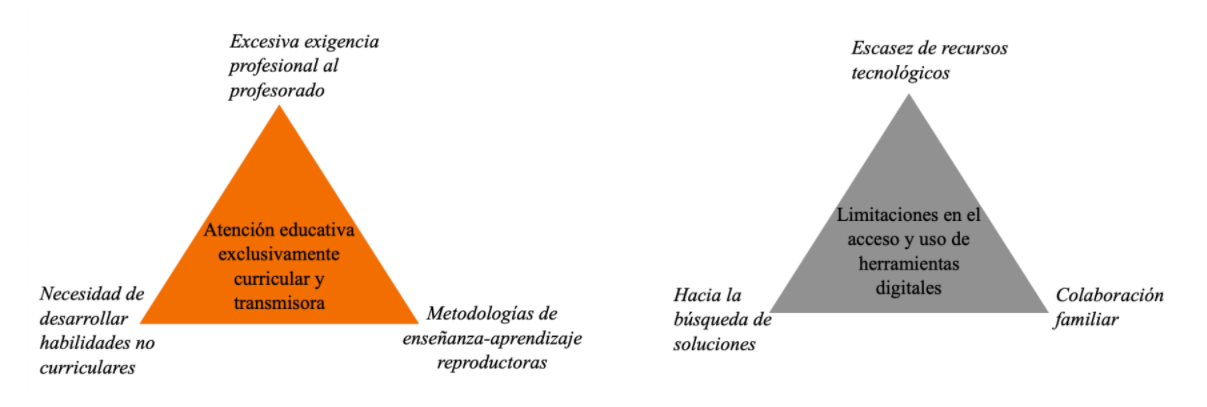
\includegraphics[width=0.95\textwidth]{figura.png}
 \caption{Categorías analíticas y subcategorías.}
 \label{fig1}
 \source{Elaboración propia.}
\end{figure}

En las próximas páginas profundizamos en las categorías de análisis haciendo uso de los resultados obtenidos en forma de evidencias (fragmentos de las entrevistas y de los grupos de discusión).

\section{Discusión}
\subsection{Atención educativa exclusivamente curricular y transmisora}
Desde una dimensión curricular, social y emocional, el alumnado con NEAE precisa de metodologías, recursos, estrategias y actividades activas, dinámicas, manipulativas, cooperativas y adaptadas a sus necesidades, intereses y potencialidades \cite{gonzalez2020}. %(GONZÁLEZ, 2020).
Sin embargo, y como consecuencia de las limitaciones inherentes a la educación telemática, a la carga de trabajo asignada al profesorado especialista y a la escasa formación del profesorado para adaptar contenido y actividades a la enseñanza virtual, estos alumnos/as (1) han recibido durante el periodo de confinamiento una atención educativa centrada exclusivamente en el desarrollo del currículum escolar, y (2) los docentes han recurrido principalmente a metodologías de enseñanza-aprendizaje transmisoras y reproductoras vinculadas con actividades de “papel y lápiz”.  

\begin{quote}
\emph{La dinámica general de trabajo adoptada en mi caso fue la propuesta de una serie de tareas semanales basadas en el refuerzo y afianzamiento de objetivos y contenidos curriculares considerados prioritarios que he ido enviando diariamente por correo electrónico} (entrevista, MGP).

\emph{Comencé la primera parte del confinamiento enviándoles un plan de trabajo diario a las familias con enlaces a actividades interactivas de lecturas comprensivas, gramática y expresión escrita, actividades interactivas de conocimiento del medio y sociales y vídeos explicativos. Así como enlaces a juegos de atención y memoria. También sus fichas correspondientes a cada unidad didáctica} (entrevista, MTGO).

\emph{He priorizado el trabajo en las áreas de Lengua, Matemáticas, Ciencias Sociales, Ciencias Naturales e Inglés con tareas de leer y responder preguntas, intenté utilizar classroom o genially pero no conseguí nada interesante y desistí, también me costaba mucho adaptar las clases y los materiales a modo virtual} (grupo de discusión, NMV).

\emph{Mi sensación durante el confinamiento ha sido de saturación, tenía 13 alumnos, he tenido que buscar, adaptar y enviar el material diariamente a cada alumno, elaborar un documento con fechas, actividades, alumnado y dificultades que he ido encontrando, preparar las clases virtuales para explicar dudas, descargarme y aprender a utilizar aplicaciones nuevas, entre otras muchas cosas, y apenas he tenido tiempo para trabajar habilidades o destrezas más prácticas y vinculadas con los Programas específicos} (entrevista, MAS). 
\end{quote}

Nos encontramos con profesorado que aún teniendo ordenadores equipados y actualizados no disponen de las aplicaciones y del conocimiento para adaptar su metodología a plataformas de comunicación sincrónicas que le permitan impartir docencia y desarrollar los Programas Específicos. Esta limitación del profesorado en el uso de herramientas digitales ha reducido “el proceso de enseñanza-aprendizaje” al envío y recepción de material curricular vía correo electrónico, evidenciando la escasa capacidad y formación de algunos docentes para adaptar a la docencia telemática la presentación y adaptación de los contenidos, la metodología, la supervisión de las tareas y la evaluación individualizada del alumnado con NEAE.

Como se infiere de los relatos del profesorado especialista en atención a la diversidad, la enseñanza telemática ha mostrado no ser efectiva, pues el alumnado con NEAE precisa de metodologías que promocionen la manipulación, la interacción y la cooperación, de un seguimiento individualizado que no es factible sin la presencialidad, de materiales y entornos adaptados \cite{rogero2020} %(ROGERO, 2020) 
y de orientación, tutorización, guía y vínculo \cite{munoz2020}. %(MUÑOZ; LLUCH, 2020)
Como señalan algunos docentes, el trabajo con el alumnado con NEAE requiere de una serie de estrategias y principios pedagógicos y de una complicidad e implicación personal y emocional que difícilmente se pueden poner en práctica sin la presencialidad.

\begin{quote}
\emph{He tenido que bajar el nivel de exigencia de las actividades, empecé enviando actividades similares a las que veníamos haciendo en clase antes del confinamiento, pero algunas familias me decían que eran muy difíciles para sus hijos. Esto es entendible porque nosotros en clase hacemos muchas actividades previas que facilitan el trabajo de los alumnos} (grupo de discusión, ACF).

\emph{El niño o niña con necesidades precisa de que el maestro esté delante, esa educación de proximidad, esa cercanía, esas distancias cortas, el perfil de nuestro alumnado precisa de estar con ellos, no de clases virtuales, por ese vínculo afectivo, educativo y curricular, de que le expliquemos y de que sea una atención más personalizada} (entrevista, CVG).
\end{quote}

A lo largo del periodo de confinamiento han sido muchos los esfuerzos realizados por el profesorado para adaptar los contenidos y las metodologías y por las familias para responder a las demandas escolares \cite{rogero2020}. %(ROGERO, 2020)
Sin embargo, la atención educativa que ha estado recibiendo el alumnado con NEAE para desarrollar competencias y habilidades comunicativas, cognitivas, sociales, etc., por parte del profesorado de Pedagogía Terapéutica (metodologías activas, recursos manipulativos e interactivos, Programas Específicos de Habilidades sociales, procesos psicológicos básicos, habilidades lectoescritoras, etc.), ha sido eliminada o limitada a intervenciones virtuales y puntuales. Esto se debe a que su desarrollo requiere de (1) actuaciones presenciales y personalizadas (2) una serie de estrategias y conocimientos específicos (de los que las familias no disponen), (3) materiales adaptados a cada una de las sesiones, y (4) una organización escolar y metodológica particular que no siempre se ha podido desarrollar de manera virtual.

\begin{quote}
\emph{Aunque he estado adaptando materiales con la página liveworksheets y les he dicho a las familias que se descarguen algunas aplicaciones para trabajar la atención y la memoria, no ha servido de mucho. Creo que no ha funcionado porque nuestro trabajo requiere de una serie de conocimientos, de una planificación y organización específica de las sesiones y de material que adaptamos y personalizamos para nuestros alumnos, y eso por mucho que lo expliques no es fácil de hacer, porque si yo veo que una actividad no funciona con un alumno puedo pasar a otra que sé que le motiva más y lo engancho, eso la familia no puede hacerlo} (grupo de discusión, FGA).

\emph{Con los alumnos de infantil, evidentemente totalmente dependientes ante las TIC, ha sido imposible trabajar conceptos básicos puesto que las familias tampoco podían prestar toda la atención que necesitaban. Los niños/as han perdido hábitos, normas, rutinas y muchos contenidos, cuando hablo con los compañeros, la frase más repetida es “un año perdido”} (entrevista, ABMG).

\emph{He mantenido mi grupo de alumnos de habilidades sociales a través de la plataforma zoom, pero me he encontrado con muchas limitaciones, en general no querían participar y no contestaban a muchas de las preguntas} (entrevista, LOD).
\end{quote}

A pesar de los enormes esfuerzos realizados por el profesorado especialista para continuar con su rutina de trabajo durante el confinamiento y de la complejidad de desarrollar de forma telemática las sesiones, encontramos una serie de limitaciones profesionales que son clave para entender por qué estas actuaciones no han tenido los resultados previstos. Como nos recuerda \textcite{fernandezdomingues2020}, %Fernández, Domínguez y Martínez (2020)
los buenos docentes no han de serlo también a través de los medios telemáticos, pues el uso que el profesorado realiza de las diferentes tecnologías responde a la formación, experiencia y perspectiva particular de cada profesional \cite{marin2020}. %(MARÍN; VAGENA; RUBIO, 2020). 

En este sentido, hemos de considerar que la enseñanza virtual precisa de la adaptación de materiales a los entornos virtuales \cite{berastegui2020}, %(BERASTEGUI, 2020),
de mejorar la competencia digital del profesorado y de una organización que ajuste la metodología y la evaluación a esta modalidad, aspectos que en gran medida precisan de formación. El principal motivo por el que muchas de las actividades propuestas por el profesorado no han funcionado son consecuencia (1) del poco conocimiento de estrategias de enseñanza virtual y de la escasa disponibilidad de contenidos adaptados a estos contextos \cite{rogero2020} %(ROGERO, 2020) 
y, (2) de la escasa oferta de materiales y plataformas virtuales adaptadas al alumnado con NEAE.

Otro de los aspectos limitantes ha sido que durante el periodo de confinamiento el profesorado se ha encontrado saturado para responder de un modo personalizado a las necesidades del alumnado con discapacidad \cite{vega2020}. %(VEGA, NAVARRO, PÉREZ Y GUERRERO, 2020)
Esta percepción responde a una dimensión externa caracterizada por la excesiva burocracia que se le ha exigido al profesorado, las continuas convocatorias de reuniones y la enorme carga de trabajo asociada a tener que dar una respuesta ajustada y personalizada a cada uno de los alumnos y alumnas diariamente, aspectos que han contribuido a mermar la capacidad pedagógica de los docentes y a limitar el tiempo disponible para preparar y adaptar las clases al formato virtual. 

\begin{quote}
\emph{Estaba desbordada, entre las reuniones de ciclo, reuniones con la orientadora y con las familias y la enorme cantidad de documentos que he tenido que completar para hacer un registro, apenas tenía tiempo de preparar material} (grupo de discusión, NMV).

\emph{Con el equipo de orientación hubo mucha coordinación a través del chat del WhatsApp, teníamos los días repartidos para atender al alumnado y estábamos en coordinación constante y un drive donde subíamos semanalmente la programación} (entrevista, BCM).

\emph{Como la comunicación era con las madres (siempre fueron las madres las que respondían) a través del WhatsApp, ellas no respetaban ningún horario, por lo que me devolvían el trabajo de sus hijos (fotos por teléfono y correo electrónico), a cualquier hora y cualquier día de la semana} (entrevista, CGR).
\end{quote}

Los docentes son conocedores que la atención educativa que se le ha ofrecido al alumnado con NEAE a lo largo del confinamiento no ha sido la deseada. Como se desprende de las evidencias y de los análisis realizados, esto se ha debido a una serie de dimensiones internas (formación del profesorado en el manejo de TIC, dificultades para adaptar las sesiones y el material a las sesiones virtuales…) y externas (responder a las demandas solicitadas por los centros educativos, el alumnado y las familias, utilizar materiales, actividades y plataformas adaptadas a las necesidades del alumnado…) que han limitado la atención educativa a procesos de enseñanza expositivos, memorísticos y repetitivos. Sin embargo, hemos de considerar que existen algunos contenidos y habilidades del currículum que difícilmente se pueden trabajar de un modo telemático, no obstante, y como venimos señalando, el aprendizaje no se puede limitar a prácticas de enseñanza-aprendizaje asentadas en un paradigma transmisor-reproductor y de educación depositaria \cite{freire1970}. %(FREIRE, 1970). 

\subsection{Limitaciones en el acceso y uso de herramientas digitales}
Si como indica \textcite[p. 176]{rogero2020}, %Rogero (2020, p. 176)
(a) el acceso a dispositivos digitales, (b) el conocimiento sobre su uso y (c) la disponibilidad de contenidos y metodologías adaptados al aprendizaje a distancia han supuesto una limitación para los estudiantes de un modo general. En el caso del alumnado con discapacidad, su falta de destreza, competencias y/o la poca accesibilidad que ofrecen las principales aplicaciones han limitado su uso por parte de este colectivo \cite{murillo2020}. %(MURILLO; DUK, 2020). 

En relación con la primera idea, algunas evidencias al respecto: \emph{“en ocasiones las familias no contaban con los medios tecnológicos necesarios”} (entrevista, ABMG), \emph{“ni siquiera tenía ordenador, ni Tablet”} (entrevista, BCM), \emph{“algunos alumnos no podías acceder al material y a las clases on line porque o no tenían internet o el único dispositivo que tenían era el móvil de sus padres y no coincidían las horas”} (MESV), \emph{“una de las alumnas solo contaba con un ordenador familiar”} (entrevista MTGO). Como hemos señalado anteriormente, la brecha digital ha sido una de las dimensiones limitantes, en este sentido, son muchas las casuísticas que nos han descrito los y las participantes (familias sin ordenador en casa, que tienen que compartir un ordenador entre todos sus miembros, que no tienen conexión a Internet o que solo tienen el móvil familiar) y que en gran medida han limitado las opciones de aprendizaje del alumnado con NEAE durante el periodo de confinamiento.  

En relación con la disponibilidad de recursos técnicos y como han expresado muchos docentes, los equipos directivos de los centros educativos se han responsabilizado de contactar con las familias que no disponían de medios tecnológicos y de dotarlas temporalmente de ordenadores portátiles y dispositivos USB de conexión inalámbrica a internet. Sin embargo, no todos los centros educativos han dispuesto de estos recursos, lo que ha promovido que instituciones como los ayuntamientos hayan tomado otro tipo de medidas para hacerle llegar el material al alumnado.

\begin{quote}
\emph{Los primeros días del confinamiento desde la dirección de mi instituto se pusieron en contacto con las familias de dos alumnos míos que no tenían recursos y le cedieron ordenadores portátiles y un lápiz con conexión a internet} (entrevista, AGM). 

\emph{Precisamente con un alumno fue un caos al principio porque eran tres hermanos en edad escolar y solo tenían un ordenador, finalmente desde el ayuntamiento le cedieron un ordenador portátil a este alumno porque el colegio no tenía más ordenadores} (grupo de discusión, AST).

\emph{Cabe destacar el caso de un alumno sin conexión a Internet en casa y con el que únicamente podía trabajar de forma telefónica, esto fue en parte posible gracias a la colaboración del ayuntamiento y la policía local quienes imprimieron e hicieron llegar al alumno el material que el profesorado había preparado} (entrevista, MGP).
\end{quote}

Como nos recuerda \textcite{mur2016}, %Mur (2016)
la brecha digital no ha sido el único problema al que nos hemos enfrentado, pues las necesidades y/o limitaciones (físicas, cognitivas, comunicativas…) que muestran algunos de los alumnos y alumnas con NEAE en el acceso y uso de dispositivos y herramientas digitales ha requerido del compromiso y de la participación activa de las familias como canal de comunicación y atención educativa del alumnado, de este modo lo expresan algunos docentes:

\begin{quote}
\emph{Los alumnos/as del primer ciclo de educación primaria no manejaban bien las plataformas como Moodle o Classroom y las familias hacían lo que podía porque estaban saturadas de trabajo, actividades, obligaciones y todo ello en el contexto que se estaba viviendo} (entrevista, ABMG).

\emph{El trabajo con el alumnado del aula específica durante el confinamiento ha sido muy laborioso y pesado. Ninguno tenía la competencia digital necesaria para trabajar online. Únicamente con una alumna con Discapacidad visual y motora me resultó fácil y asequible trabajar con ella, puesto que la madre estaba todo el tiempo con nosotras y me hizo más fácil llevar la clase} (entrevista, BCM).

\emph{Me he encontrado de todo, desde familias que han podido compaginar su trabajo y ayudar a sus hijos a conectarse y a ayudarle a manejar el ordenador y las aplicaciones, hasta familias que no han podido ayudar por motivos de trabajo, que no sabían manejar el ordenador o que no querían} (grupo de discusión, RMG).

\emph{Nunca puede sustituir las clases presenciales a las clases online, al menos para el perfil del alumnado al que yo atiendo, en mi caso al menos, su nivel de autonomía personal es muy bajo, no pudiendo ellos por sí solos ponerse frente a un ordenador} (entrevista, MTGO).
\end{quote}

Como evidencian \textcite{vega2020}, %Vega, Navarro, Pérez y Guerrero (2020)
las limitaciones que presentan los estudiantes con discapacidad para hacer uso de dispositivos tecnológicos están vinculadas (1) con las competencias digitales y destrezas del alumnado, y (2) con la accesibilidad a los entornos virtuales que ofrecen los programas informáticos. Ambas dimensiones han sido señaladas por el profesorado como unas de las grandes dificultades a las que se han enfrentado durante el confinamiento tanto ellos, las familias, como el alumnado.

\begin{quote}
\emph{No tenían conocimientos digitales, ni siquiera tenía ordenador, ni Tablet. Les intenté enseñar a usar el correo y les costó mucho, pero finalmente fueron recibiendo alguna tarea por ese medio} (entrevista, BCM).

\emph{Mis alumnos no tienen capacidad para manejar el ordenador de forma autónoma y mucho menos para abrir un correo, un enlace y utilizar zoom, ellos han sido totalmente dependientes de sus padres. Es un error que no se les enseñe en el colegio a utilizar estas herramientas} (entrevista, MRF).

\emph{Aunque algunas plataformas son muy intuitivas y aparentemente fáciles de utilizar, tienen muchas opciones y no están adaptadas para el alumnado con discapacidad} (entrevista, JFRD).
\end{quote}

La escasa accesibilidad que presentan la mayoría de páginas webs y aplicaciones \cite{renilla2010} %(RENILLA: PEDRERO; SÁNCHEZ, 2010) 
y los principales entornos digitales de comunicación, unido a la poca formación que desde los contextos educativos se le ha venido ofreciendo al alumnado con NEAE para utilizar de forma autónoma las TIC, han sido los dos principales factores que han limitado el uso de estas tecnologías de manera autónoma por parte del alumnado con NEAE.

Rescatando una idea anteriormente mencionada, nos hemos encontrado, por un lado, con una brecha de acceso o brecha digital, vinculada con el acceso a recursos tecnológicos e internet, y, por otro lado, con una brecha de uso relacionada con la utilización de las tecnologías \cite{rogero2020}. %(ROGERO, 2020).
Sin embargo, y en el caso particular del alumnado con NEAE, hemos asistido también a una brecha vinculada con la adaptación y accesibilidad de las plataformas y aplicaciones digitales. 

\section{A modo de conclusión}
Las narraciones de los docentes han evidenciado una serie de dimensiones que creemos que son clave para entender las debilidades o limitaciones que el sistema educativo ha mostrado a lo largo del periodo de confinamiento para con el alumnado con NEAE, con todo lo que esto significa y engloba. A modo de conclusión abordamos dos reflexiones que emergen de esta investigación, y que a nuestro juicio son retos que las administraciones educativas deben afrontar:

\begin{itemize}
    \item \emph{Necesidad de crear herramientas digitales más accesibles.} 
    La etapa educativa y/o el nivel de competencia curricular del alumnado con NEAE va a determinar en gran medida la metodología utilizada en los contextos virtuales \cite{menendez2020}. %(MENÉNDEZ; FIGARES, 2020).
    Sin embargo, y a pesar del esfuerzo realizado por el profesorado, las necesidades particulares de estos alumnos y alumnas han demandado durante el periodo de docencia telemática de materiales, aplicaciones y metodologías adaptadas a sus características y de adaptaciones tecnológicas personalizadas. Como señalan al respecto \textcite{vega2020}, %Vega, Navarro, Pérez y Guerrero (2020)
    la mayoría de estudiantes con NEAE no dispone de destrezas para manejar las principales aplicaciones utilizadas por el profesorado debido a que sus entornos virtuales no son accesibles. Esta situación, que desafortunadamente ha sido más habitual de lo deseado, ha tenido consecuencias para el alumnado con NEAE que, o bien no ha podido acceder de manera autónoma al material escolar (videos, clases, actividades, foros…), o bien ha necesitado de la ayuda de un familiar para poder atender a sus obligaciones escolares. 
    
    \item \emph{Mejorar la formación del profesorado y del alumnado.} 
    Si algo nos ha demostrado la formación virtual, es que existe, además de una brecha digital, una brecha de uso \cite{fernandezenguita2020} %(FERNÁNDEZ-ENGUITA, 2020)
    o brecha de competencias, que está relacionada con las competencias digitales del profesorado para utilizar, crear y compartir actividades educativas en plataformas virtuales y con las competencias del alumnado para acceder y trabajar con material digital e interactuar en escenarios virtuales \cite{garciapenalvo2020}. %(GARCÍA-PEÑALVO; ABELLA-GARCÍA; CORELL; GRANDE, 2020).
    Esta situación ha obligado a profesorado y alumnado a utilizar aplicaciones y recursos digitales sin una formación previa \cite{rogero2020}. %(ROGERO, 2020)
    Las limitaciones evidenciadas por el profesorado y el alumnado en el uso de recursos virtuales interpelan a las administraciones competentes, por un lado, a realizar un esfuerzo para mejorar y ampliar la oferta formativa para el profesorado a partir de itinerarios y programas formativos acordes a las necesidades detectadas (organizativas, metodológicas, didácticas, evaluadoras…); por otro lado, a ampliar la formación competencial digital del alumnado extendiendo la asignatura Cultura y práctica digital (que se cursa exclusivamente en sexto de primaria en la comunidad autónoma de Andalucía) a la totalidad del alumnado de Educación primaria.
\end{itemize}

Estamos ante dos retos microsistémicos que requieren de una respuesta compleja, concreta y comprometida por parte de las administraciones educativas competentes. Sin embargo, si queremos abordar con garantías el objetivo de desarrollo sostenible cuatro, garantizar una educación inclusiva, equitativa de calidad y promover oportunidades de aprendizaje permanente para todos \cite[p. 16]{onu2015}, %(ONU, 2015, p.16)
propuesto por las Naciones Unidas en la agenda 2030, hemos de dar respuesta a estos retos de una manera eficaz. En este sentido, esta experiencia nos ha demostrado que necesitamos replantearnos las prácticas educativas virtuales que se han venido desarrollando a lo largo del periodo de confinamiento, y con esa experiencia, diseñar actividades, metodologías, recursos…, que consideren el grado de autonomía, conocimiento y desarrollo del alumnado hacia el que va dirigida \cite{moreno2020}. %(MORENO, 2020).

Este trabajo evidencia la invisibilidad que existe en el ámbito de la atención a la diversidad en cuanto a uso de TIC se refiere. De un modo particular, es también un dato significativo la insuficiente investigación que se ha realizado sobre el impacto que la COVID-19 ha tenido en el proceso formativo del alumnado con discapacidad \cite[p. 7]{vega2020}. %(VEGA, NAVARRO, PÉREZ Y GUERRERO, 2020, p. 7).
Esta situación es aún más preocupante cuando aludimos a investigaciones en la que participen profesorado especialista de atención a la diversidad o alumnado con necesidades educativas. No obstante, esta investigación, aunque acotada en la comunidad andaluza y con una muestra de participantes no representativa para generalizar los resultados obtenidos, nos ofrece una panorámica de las principales dificultades y limitaciones a las que se ha enfrentado el profesorado especialista de Pedagogía Terapéutica. 

\printbibliography\label{sec-bibliography}
% if the text is not in Portuguese, it might be necessary to use the code below instead to print the correct ABNT abbreviations [s.n.], [s.l.] 
%\begin{portuguese}
%\printbibliography[title={Bibliography}]
%\end{portuguese}

\end{document}
